\documentclass[12pt,oneside]{uhthesis}
\usepackage{subfigure}
\usepackage[ruled,lined,linesnumbered,titlenumbered,algochapter,spanish,onelanguage]{algorithm2e}
\usepackage{amsmath}
\usepackage{amssymb}
\usepackage{bookmark}
\usepackage{amsbsy}
\usepackage{caption,booktabs}
\captionsetup{ justification = centering }
% \usepackage{mathpazo}
\usepackage{float}
\setlength{\marginparwidth}{2cm}
\usepackage{todonotes}
\usepackage{listings}
\usepackage{xcolor}
\usepackage{multicol}
\usepackage{graphicx}
\floatstyle{plaintop}
\restylefloat{table}
\addbibresource{Bibliography.bib}
% \setlength{\parskip}{\baselineskip}%
\renewcommand{\tablename}{Tabla}
%\dontprintsemicolon
\SetAlgoNoEnd



\definecolor{codegreen}{rgb}{0,0.6,0}
\definecolor{codegray}{rgb}{0.5,0.5,0.5}
\definecolor{codepurple}{rgb}{0.58,0,0.82}
\definecolor{backcolour}{rgb}{0.95,0.95,0.92}

\lstdefinestyle{mystyle}{
    backgroundcolor=\color{backcolour},   
    commentstyle=\color{codegreen},
    keywordstyle=\color{purple},
    numberstyle=\tiny\color{codegray},
    stringstyle=\color{codepurple},
    basicstyle=\ttfamily\footnotesize,
    breakatwhitespace=false,         
    breaklines=true,                 
    captionpos=b,                    
    keepspaces=true,                 
    numbers=left,                    
    numbersep=5pt,                  
    showspaces=false,                
    showstringspaces=false,
    showtabs=false,                  
    tabsize=4
}

\lstset{style=mystyle}

\title{Generación Automática de un Borrador de Estado del Arte a partir de una colección de documentos científicos\par}
\author{\vspace{0.25cm}Javier Alejandro Oramas López}
\advisor{\vspace{0.25cm}Dr. Yudivián Almeida}
\degree{Licenciado en Ciencia de la Computación}
\faculty{Facultad de Matemática y Computación}
\date{05/01/2024\\\vspace{0.25cm}\href{https://github.com/JavierOramas/thesis\_experiments}{github.com/JavierOramas/thesis\_experiments}}
\logo{Graphics/uhlogo}
\makenomenclature

\renewcommand{\vec}[1]{\boldsymbol{#1}}
\newcommand{\diff}[1]{\ensuremath{\mathrm{d}#1}}
\newcommand{\me}[1]{\mathrm{e}^{#1}}
\newcommand{\pf}{\mathfrak{p}}
\newcommand{\qf}{\mathfrak{q}}
%\newcommand{\kf}{\mathfrak{k}}
\newcommand{\kt}{\mathtt{k}}
\newcommand{\mf}{\mathfrak{m}}
\newcommand{\hf}{\mathfrak{h}}
\newcommand{\fac}{\mathrm{fac}}
\newcommand{\maxx}[1]{\max\left\{ #1 \right\} }
\newcommand{\minn}[1]{\min\left\{ #1 \right\} }
\newcommand{\lldpcf}{1.25}
\newcommand{\nnorm}[1]{\left\lvert #1 \right\rvert }

\begin{document}

\frontmatter
\maketitle

\begin{dedication}
    A mi abuela Mirtha, que hubiera querido estar aquí hoy, como tantas otras veces, para celebrar un logro de su nieto \emph{`científico'}
\end{dedication}
\begin{acknowledgements}
    En primer lugar le agradezco a mi tutor, el profesor Yudivian, y al resto de profesores de la facultad, por siempre obligarme a dar lo mejor de mi. Al profesor Rodrigo Cuéllar Hidalgo, la maestra Micaela Chávez y la doctora Mayra Mena, por acogerme en el Colegio de México, donde realicé parte importante de esta investigación.
    
    A mis amigos Isabel, Daniel y Lia, por haberme ayudado a superar los momentos más dificiles de la carrera. Junto a ustedes he alcanzado los logros profesionales que más me enorgullecen. Al resto de amistades que, si no los menciono, sepan que los aprecio.

    A mi familia, mis padres, que han sido un apoyo constante durante todos estos años. Han sido mis consejeros, editores y lo que fuere que amerite la situación. Sin ustedes esto no hubiese sido posible.
    
    A mis Tíos y abuelos, que siempre se mantuvieron al tanto de mi, y estaban siempre ávidos de ayudar. A mis abuelos, los que ya no están, por ser motivación constante. A Alejandra, mi compañera, mi soporte, por simepre estar dispuesta a darme fuerzas cuando más lo necesito.

    A los que no menciono, pero contribuyeron directa o indirectamente a que hoy esté aquí. Gracias a todos.
\end{acknowledgements}
\include{FrontMatter/SupervisorOpinion}
\begin{resumen}
	En la actualidad, la gestión eficiente de la vasta cantidad de documentos científicos vinculados a un tema específico se ha convertido en un desafío creciente. Este estudio propone un pipeline diseñado para optimizar dicho proceso, abordándolo en tres etapas esenciales. Primero, se enfoca en la detección de los aspectos más relevantes dentro de la bibliografía proporcionada. Luego, se procede a la generación de un resumen abstractivo que condensa la información asociada con cada aspecto identificado, integrando referencias a los documentos pertinentes para respaldar la información presentada. Finalmente, se realiza una abstracción general del texto generado, proporcionando una visión consolidada de la información extraída.

	La evaluación de este enfoque se lleva a cabo mediante el análisis de resultados utilizando conjuntos de datos específicamente diseñados para el procesamiento de múltiples documentos. Este proceso de evaluación busca validar la efectividad y la precisión del pipeline propuesto en la identificación y síntesis de información relevante a partir de documentos científicos extensos. Con esta investigación, se busca no solo mejorar la eficiencia en la revisión de la literatura científica, sino también proporcionar una herramienta valiosa para investigadores y profesionales que enfrentan el desafío de abordar grandes volúmenes de información en sus respectivos campos.
\end{resumen}

\begin{abstract}
	Currently, the efficient management of the vast amount of scientific documents associated with a specific topic has become an increasingly challenging task. This study proposes a pipeline designed to streamline this process, addressing it in three essential stages. First, it focuses on detecting the most relevant aspects within the existing literature. Next, it proceeds to generate an abstractive summary that condenses information associated with each identified aspect, integrating references to pertinent documents to support the presented information. Finally, a general abstraction of the generated text is performed, providing a consolidated view of the extracted information.

	The evaluation of this approach is carried out by analyzing results using datasets specifically designed for processing multiple documents. This evaluation process aims to validate the effectiveness and accuracy of the proposed pipeline in identifying and synthesizing relevant information from extensive scientific documents. With this research, the goal is not only to improve efficiency in reviewing scientific literature but also to provide a valuable tool for researchers and professionals facing the challenge of addressing large volumes of information in their respective fields.
\end{abstract}
\tableofcontents
% \listoffigures
% \listoftables
% \listofalgorithms
% \lstlistoflistings

\mainmatter

\chapter*{Introducción}\label{chapter:introduction}
\addcontentsline{toc}{chapter}{Introducción}

    El vertiginoso flujo de producción de artículos científicos en la actualidad plantea un desafío sustancial: la imposibilidad práctica de revisar exhaustivamente todos los documentos relacionados con una investigación. Solo en \emph{ArXiv}\footnote{ArXiv es un repositorio en línea donde los investigadores comparten artículos académicos antes de la revisión por pares y la publicación formal.}, se registran alrededor de 180,000 nuevas (pre) publicaciones por año [\cite{arxivstats}]. Esta abrumadora cantidad de información subraya la necesidad imperante de encontrar enfoques eficientes para obtener resúmenes de documentos científicos, una problemática que ha sido abordada a lo largo de los años mediante diversos intentos de automatización.

    La historia de los resúmenes automáticos se remonta a las décadas de 1950 y 1960, cuando la inteligencia artificial (\emph{IA}) comenzó a surgir como un campo de investigación. Desde este período, los científicos se centraron en el procesamiento del lenguaje natural (\emph{NLP} por sus siglas en inglés) como un componente clave para desarrollar sistemas de resumen. Uno de los hitos tempranos fue el trabajo de Hans Peter Luhn en 1958 [\cite{luhun1958}], quien propuso un método para extraer automáticamente oraciones clave de un documento basado en la frecuencia de las palabras clave. Este enfoque inicial estableció las bases para futuras investigaciones en resúmenes automáticos.

    Con el avance de las investigaciones surgieron enfoques más sofisticados: algoritmos basados en grafos, como \emph{TextRank} [\cite{mihalcea2004textrank}], los cuales se convirtieron en una herramienta valiosa para la extracción de información. Las investigaciones también han explorado enfoques supervisados [\cite{collins-etal-2017-supervised}], donde se utilizan técnicas de clasificación de oraciones, y se han abordado desafíos tanto en su comprensión como en la generación de lenguaje. [\cite{knight2000statistics}]

    Se ha experimentado un significativo avance con el desarrollo de los algoritmos de extracción y abstracción de información. Estos enfoques fundamentales definen cómo los sistemas automáticos condensan la información de un texto, ya sea seleccionando oraciones del texto original o generando un texto totalmente nuevo que contenga la información del original de manera más concisa.

    Los algoritmos de extracción, al seleccionar oraciones de la fuente de información, presentan ventajas notables. En principio, conservan la información original, y son especialmente útiles en contextos donde la fidelidad a los hechos es esencial, como en informes científicos o noticias. Además, al evitar la generación de lenguaje nuevo, estos enfoques minimizan el riesgo de errores gramaticales y son computacionalmente eficientes. Sin embargo, su limitación radica en la falta de creatividad y generalización, dependiendo exclusivamente de la información presente en el texto original, al tiempo que puede conducir a resúmenes redundantes [\cite{LexRank}]

    En oposición a la extracción, los algoritmos de abstracción buscan generar una redacción nueva, ofreciendo creatividad y capacidad de generalización. Esta capacidad de expresar la esencia del contenido de manera única es una ventaja clave [\cite{rush2015neural}]. Además, la abstracción puede manejar información no presente de manera literal en el texto original, permitiendo una expresión más amplia de ideas [\cite{PaulusXS17}]. Sin embargo, los modelos con este enfoque enfrentan desafíos significativos tanto en la generación de lenguaje como en la posibilidad de incurrir en errores gramaticales o falta de coherencia. También existe el riesgo de introducir sesgos, dependiendo de la calidad del modelo y de los datos de entrenamiento. La abstracción suele ser más compleja computacionalmente en comparación con la extracción.

    No obstante, existen también enfoques híbridos [\cite{SeeLM17}], ya sea integrando técnicas de extracción y abstracción, o  combinaciones de diferentes enfoques dentro de un marco unificado. Estos enfoques buscan aprovechar las fortalezas de cada método para mejorar la calidad y la diversidad de los resúmenes generados.

    Este enfoque más amplio no solo aborda la creciente complejidad asociada con la información dispersa, sino que también presenta potencialidades para mejorar la coherencia temática y la comprensión integral de un tema al considerar múltiples perspectivas y contextos.

    Históricamente, la mayoría de los enfoques en el campo del resumen automático se han orientado hacia la generación de resúmenes para un solo documento, buscando condensar la información esencial de manera concisa. Sin embargo, a medida que la era digital ha transformado la forma en que accedemos a la información, la investigación más reciente ha dirigido su atención hacia la generación de resúmenes de múltiples documentos. Este cambio estratégico se ha vuelto esencial en entornos donde la información relevante se distribuye en diversas fuentes, como es el caso de la generación de resúmenes de noticias [\cite{fabbri2019multi-news}], la síntesis de artículos de Wikipedia [\cite{liu2018}], y la producción de resúmenes tipo \emph{Estado del arte}\footnote{Un estado del arte es una revisión exhaustiva y actualizada de los avances, investigaciones y desarrollos existentes en un campo específico de estudio o disciplina, que proporciona una visión panorámica de la situación actual del conocimiento en ese ámbito. } para documentos científicos [\cite{lu2020multixscience}].

    La generación de resúmenes de múltiples documentos no se limita simplemente a la agregación de información; más bien, implica la síntesis de conocimientos interconectados para ofrecer una visión holística. 
    Estos avances reflejan la adaptación dinámica de los métodos de resumen automático para satisfacer las demandas cambiantes de la era digital y para abordar la abundancia de información interrelacionada que caracteriza el entorno actual de la investigación y la comunicación científica.

    Los Modelos de Lenguaje con Aprendizaje Profundo (LLM, por sus siglas en inglés) han emergido como elementos cruciales para la generación de resúmenes automáticos. Los LLM, han demostrado una capacidad excepcional para entender la semántica y la estructura del lenguaje [\cite{fewshot}]. Su entrenamiento masivo en grandes corpora\footnote{Conjunto de datos, textos u otros materiales sobre determinada materia que pueden servir de base para una investigación o trabajo.} de texto les permite capturar patrones complejos y generar resúmenes coherentes y contextualmente relevantes.

    Las ventajas de los LLM en este contexto son notables. En primer lugar, su capacidad para comprender el significado contextual permite generar resúmenes que no solo seleccionan información clave, sino que también la expresan de manera más fluida y comprensible [\cite{Radford2018ImprovingLU}]. Además, los LLM pueden abordar la generación de lenguaje nuevo de manera más efectiva, superando algunos desafíos asociados con la abstracción, como errores gramaticales y falta de coherencia [\cite{RoBERTa}].

\section{Motivación}
    Es evidente la necesidad de crear una herramienta que permita a los investigadores procesar grandes cantidades de texto de manera eficiente y rebasar las limitaciones que actualmente suponen tanto el tiempo de lectura de artículos científicos como el volumen de información sobre cada tema para la creación de estados del arte en investigaciones científicas

    Si bien existen algunos sistemas  [\cite{elicit},\cite{scite}], que permiten la extracción de información de múltiples documentos, por lo general requieren de un conocimiento previo de los temas que tratan. Además, la interacción en escencia se presenta en formato de preguntas-respuestas que, si bien puede ser deseable en algunos casos, puede hacer más tedioso el proceso de obtener de manera clara la información que se desea. Además, estos sistemas dependen de la correcta comprensión por parte del modelo de las preguntas que se le realizan.\par

\section{Problemática}
    Al hacer un estudio del estado del arte en torno a los sistemas de generación de resúmenes enfocados a la construcción de los propios estados del arte, no se encontraron modelos o metodologías públicas que sean capaces de generar textos semántica y sintácticamente correctos, y que a su vez cuenten con un sistema de citación robusto que cumpla con los requisitos de un estado del arte. Todos los candidatos encontrados resultaron deficientes en, al menos, una categoría.

\section{Hipótesis}
    Es posible desarrollar un sistema (herramienta) de generación de un borrador de estado del arte que tenga como base de conocimientos un grupo de documentos previamente seleccionados y que, a su vez, genere un texto resumen que abarque un grupo de los temas (autodetectados) más relevantes. Además, el sistema deberá ser capaz de generar citas bibliográficas de manera automática, correcta y en el formato adecuado, cumpliendo con una estructura determinada.

\section{Objetivos}
    \subsection{Objetivo General}

        Proponer un modelo que permita generar un texto que contenga una enumeración de los principales temas encontrados en el corpus de documentos; seguidos cada uno por un resumen de los contenidos `relacionados con el tema' presentes en el \emph{dataset} y con sus respectivas citaciones.

    \subsection{Objetivos Específicos}

        \begin{itemize}
            \item Definir la estructura que deberán cumplir todos los documentos generados.
            \item Proponer una metodología para la extracción de los temas principales de los documentos.
            \item Identificar o entrenar un modelo que se desempeñe satisfactoriamente en la generación de un texto que cumpla con la estructura predefinida.
            \item Realizar una validación de los resultados que permita verificar la viabilidad de el método sugerido para la generación de un texto que cumpla con los requisitos definidos.
        \end{itemize}
\section{Esbozo de solución}
    En este documento se hace una propuesta de modelo híbrido, que utiliza la representación mediante \emph{embeddings}\footnote{Un \emph{embedding} de texto es una técnica que representa palabras como vectores de números, permitiendo que palabras con significados similares tengan representaciones similares}
    de los documentos para obtener una representación vectorial del corpus, sobre la cual se trabajará para agrupar los documentos por temas. Una vez hecho esto, se obtendrán las ideas más relevantes y, mediante la utilización de un modelo de lenguaje, se modelará la información extraída para cumplir con el formato especificado.

\section{Estructura de la tesis}
        El resto del documento se encuentra organizado de la siguiente manera:

        \begin{enumerate}
            \item \emph{Capítulo 1} Se hace una revisión del estado del arte en el ámbito de la generación de resúmenes. Principalmente buscando enfoques híbridos, y modelos (o metodologías) que reduzcan los inconvenientes de los modelos clásicos.
            \item \emph{Capítulo 2} Se describe la propuesta de solución, en la que se detalla la metodología utilizada en la generación de los resúmenes.
            \item \emph{Capítulo 3} Se presentan los detalles de implementación y retos computacionales afrontados, así como la discusión y comparación de los resultados obtenidos.
            \item \emph{Capítulo 4} Se presentan conclusiones y recomendaciones para futuros trabajos.
            \item \emph{Capítulo 5} Se presentan bibliografías y anexos relacionados con la temática abordada.
        \end{enumerate}



\chapter{Estado del Arte}\label{chapter:state-of-the-art}
    Este Capítulo se centrará en dar una panorámica del estado de las investigaciones relacionadads con los resúmenes automáticos, y las herramientas necesarias para resolver problemas específicos de los enfoques con los que generan dichos resúmenes.

\section{Sistemas de Generación automática de resúmenes utilizando enfoques híbridos}

Un enfoque híbrido combina tanto las aproximaciones extractivas como abstractivas en el proceso de resumen de texto. La arquitectura típica de un summarizador de texto híbrido se muestra en la y consta comúnmente de las siguientes fases:



\begin{enumerate}
    \item Pre procesamiento.
    \item Extracción de oraciones (fase extractiva): Extraer las oraciones clave del texto de entrada\cite[(Wang et al., 2017)]{Wang}
    \item Generación del resumen (fase abstractiva): Generar el resumen final a partir de la aplicación de métodos abstractivos a las oraciones extraídas en la fase extractiva.
    \item Post Procesado: Verificar que las oraciones generadas sean válidas y se ajusten al formato deseado.
\end{enumerate}


En la propuesta de (Rasim et al., 2019)\cite{cosum} se utiliza un modelo de dos etapas que combina técnicas de clustering y optimización. En la primera etapa, se aplica el método de k-means para clusterizar las oraciones y descubrir múltiples temas en el texto. En la segunda etapa, se implementa un modelo de optimización para la selección de oraciones destacadas de los clusters. Otro enfoque interesante es el de (Ghadimi \& Beigy, 2022)\cite{hybrid-llm} que inicialmente, construye un resumen extractivo a partir de varios documentos de entrada y luego lo utiliza para generar el resumen abstractivo. La gestión de la información redundante, un problema global en la summarización de múltiples documentos, se aborda en la primera etapa, donde se utilizan similitudes basadas en BERT\cite{BERT} para calcular la redundancia de los documentos.

La incorporación de Grandes Modelos de Lenguaje (LLM) ha revolucionado el campo de procesamiento de lenguaje natural (NLP), abriendo nuevas posibilidades y elevando el rendimiento en diversas tareas, entre ellas, la sumarización de textos. En investigaciones como la realizada por (Basyal et al, 2023)\cite{basyal2023text} se observa el excepcional desempeño de los modelos de lenguaje, principalmente el modelo text-davinci-003 de OpenAI\cite{openai}. No obstante se hace la aclaración que los modelos con los que fue comparado son significativamente mas peque\~nos y se sugiere hacer uso de las versiones más complejas de los mismos.

\section{Topic Modelling}

    El análisis de texto ha experimentado avances significativos en las últimas décadas, y entre las técnicas más destacadas se encuentra el Modelado de Temas (Topic Modeling). Esta metodología, anclada en la minería de texto y el procesamiento de lenguaje natural, ha emergido como una herramienta esencial para descubrir patrones subyacentes y estructuras temáticas en grandes conjuntos de documentos. El Modelado de Temas se adentra en la complejidad de los datos textuales, permitiendo la identificación automática y la organización de temas latentes presentes en un corpus\cite{lda2003}.

    El uso de modelos basados en la arquitectura encoder-decoder se ha usado tanto para la generación de algoritmos de Topic Modelling tanto para textos cortos\cite{neuraltm} como para textos más extensos\cite{tminemb}. En todos los casos mejorando los resultados de modelos más tradicionales y ampliamente usados como Latent Dirichlet Analysis (LDA)\cite{lda2003}   

    Angelov (2020)\cite{angelov2020top2vec} presenta un nuevo modelo, que utiliza embeddings semánticos para identificar temas sin requerir parámetros predefinidos ni listas personalizadas. A diferencia de métodos tradicionales, captura la semántica de palabras y documentos, demostrando resultados más informativos y representativos en experimentos.

    \subsection{Clustering}
    Utilizando una representacion en vectores de la información a través de embeddings de texto (Sia et al. 2020)\cite{sia2020tired} presenta evaluaciones comparativas para la combinación de diferentes embeddings de palabras y algoritmos de agrupamiento. Analiza su rendimiento bajo reducción de dimensionalidad con PCA\footnote{TODO}. Mostrando en algunos casos resultados tan sólidos como los modelos de temas clásicos, pero con menor tiempo de ejecución y complejidad computacional. 
    Por esta línea se encuentra también \emph{BERTopic}\cite{bertopic} que hace una primera representación de los documentos como text embeddings, realiza clustering en el espacio de los vectores genrados y contruye los titulos de los temas utilizando un sistema de representación categórica de los temas a través de una tabla TF-IDF\footnote{TODO}

\section{Embeddings de texto}
    En la exploración de embeddings contextuales, según detalla Liu et al. (2020)\cite{liu2020survey}, el enfoque se centra en asignar representaciones a palabras basadas en su contexto, capturando sus diversos usos y codificando conocimientos transferibles entre idiomas. Su estudio profundiza en varios aspectos, incluidos los modelos existentes de embeddings contextuales, el preentrenamiento políglota entre idiomas, la aplicación de embeddings contextuales en tareas posteriores, la compresión de modelos y el análisis de modelos.

    Huang et al. (2020)\cite{Huang_2020} aportan destacan las ventajas de la aplicación de estos al ámbito de los sistemas de búsqueda, especialmente en redes sociales como Facebook. Los autores presentan un marco de recuperación basado en embeddings (EBR) y un marco de embeddings unificado para la búsqueda personalizada, exponiendo sus experiencias y optimizaciones para mejoras integrales en el sistema. Su trabajo sobre EBR en la búsqueda de Facebook muestra ganancias significativas en métricas en experimentos online.

    Reimers et al. (2022)\cite{reimers2019sentencebert} abordan la sobrecarga computacional asociada con modelos como BERT y RoBERTa en tareas de regresión de pares de oraciones. Introducen Sentence-BERT (SBERT), una modificación de BERT que utiliza estructuras de redes siamesas y tripletas para derivar embeddings de oraciones semánticamente significativos. SBERT reduce significativamente el esfuerzo computacional requerido para encontrar pares de oraciones similares, manteniendo la precisión. Su evaluación demuestra un rendimiento superior en tareas de similitud textual semántica (\emph{STS}) y tareas de transferencia en comparación con otros métodos de embedding de oraciones de última generación.

    Gao et al. (2021)\cite{gao2022simcse} contribuyen al campo con SimCSE, presentando modelos de aprendizaje contrastivo no supervisado y supervisado que mejoran significativamente los embeddings de oraciones. Su enfoque, que utiliza dropout como una mínima augmentación de datos, logra resultados destacados en tareas de similitud textual semántica (\emph{STS}). El enfoque supervisado, que incorpora pares anotados, mejora aún más la correlación, destacando la efectividad del objetivo de aprendizaje contrastivo en la regularización y alineación de los embeddings preentrenados.

    Muenninghoff et al. (2023)\cite{muennighoff2023mteb} presentan el \emph{Massive Text Embedding Benchmark (MTEB)}, una iniciativa que abarca ocho tareas de embedding, 58 conjuntos de datos y 112 idiomas. A través de la evaluación de 33 modelos en \emph{MTEB}, se establece el benchmark más completo hasta la fecha. Los resultados revelan que ningún método de embedding de texto específico domina en todas las tareas, indicando que el campo aún no ha convergido hacia un método universal. MTEB se presenta como una solución de código abierto y un\cite[leaderboard público]{leaderboard}. Este enfoque transparente y accesible contribuye a un mejor entendimiento y selección de modelos de embedding de texto, fomentando el avance y la consolidación en este campo dinámico.

\section{Modelos de Lenguaje}
   
    La influencia transformadora de las arquitecturas de transformers, introducida en "Attention is All You Need" \cite{attention}, ha sido crucial para remodelar la modelización del lenguaje. Modelos como BERT\cite{BERT} avanzaron en la comprensión bidireccional del contexto, mientras que la serie GPT (Generative Pre-trained Transformer), especialmente GPT-3\cite{brown2020language}, presentando un modelo de 175 mil millones de parámetros y su sucesor GPT4\cite{openai2023gpt4}. Otros de los modelos a destacar son el presentados por MetaAI, LLaMA(Feb. 2023)\cite{llamapaper} y LLaMA2(Jul. 2023)\cite{llamapaper2} una colección de modelos de lenguaje grandes (LLMs) preentrenados y ajustados finamente que varían en escala desde 7 mil millones hasta 70 mil millones de parámetros. Mostrando resultados prometedores en comparación con otros modelos\cite{metallama}. 
    
    \subsection{Generación de resúmenes usando LLM}

    En el trabajo de \cite[(Basyal et al. 2023)]{basyal2023text} se exploran técnicas de resumen de texto utilizando \emph{LLMs}, incluyendo MPT-7b-instruct, falcon-7b-instruct y OpenAI ChatGPT text-davinci-003. El modelo text-davinci-003 destaca como el más efectivo en diversas métricas de evaluación. Se realiza una comparación detallada en diferentes conjuntos de datos, como CNN Daily Mail y XSum, ofreciendo valiosas percepciones sobre el rendimiento de los LLMs en entornos variados. 

    \subsection{Modelos de GPT4All}

        GPT4All es un ecosistema de software libre que ha publicado un grupo de \emph{LLMs} basados en la arquitectura \emph{transformers}\cite{attention}. Los modelos GPT4All son producto de la cuantización\footnote{Cuantizar es un proceso en el cual se reduce la precisión de los números en una red neuronal, disminuyendo así los requisitos de memoria y permitiendo que modelos grandes se ejecuten en dispositivos con recursos limitados. En este contexto, cuantizar facilita el uso de modelos GPT4All en computadoras con menos capacidad de hardware.} de redes neuronales, un proceso que reduce los requisitos de VRAM VRAM\footnote{La memoria VRAM (Video Random Access Memory) es utilizada tratar los datos y las operaciones relacionadas con la tarjeta gráfica.} para ejecutar un Decodificador Transformer de varios miles de millones de parámetros. A través de algoritmos de cuantización, estos modelos pueden ser adaptados para poder ser utilizados con un hardware moderado\cite{webgpt4all}.
        
        Entre los modelos soportados se encuentran\footnote{La cantidad de parámetros especificada se refiere a los modelos cuantizados disponibles en la web de GPT4All}:
        \begin{enumerate}
            \item Falcon (7 mil millones de parámetros) \cite{falcon}
            \item LLaMA (7-13 min millones de parámetros )\cite{llama}
            \item MPT (7 mil millones de parámetros) \cite{mpt}
            \item GPT-J (6 mil millone de parámetros)\cite{gptj}
        \end{enumerate}


\chapter{Propuesta}\label{chapter:proposal}
    Para la solución de los problemas planteados se propone definir un \emph{pipeline} que contará con 6 etapas principales.
    que abarcan desde la carga de los documentos, el procesado de los mismos para ser almacenados en una base de datos. Realizar un agrupamiento para la detección de las principales temáticas presentes en el corpus y particularmente los documentos más representativos para cada una de ellas. Posteriormente estos documentos son compendiados a modo de un resumen extractivo y, a su vez, se obtienen las referencias bibliográficas correspondientes. En la ultima fase se realiza un post procesado mediante un LLM para generar un resumen abstractivo a partir del texto que se obtuvo en la fase anterior. Finalmente se junta dicho resumen con las referencias bibliograficas obtenidas. En figura () se muestra un diagrama del \emph{pipeline} descrito

    \begin{figure}[H]    
        \centering
        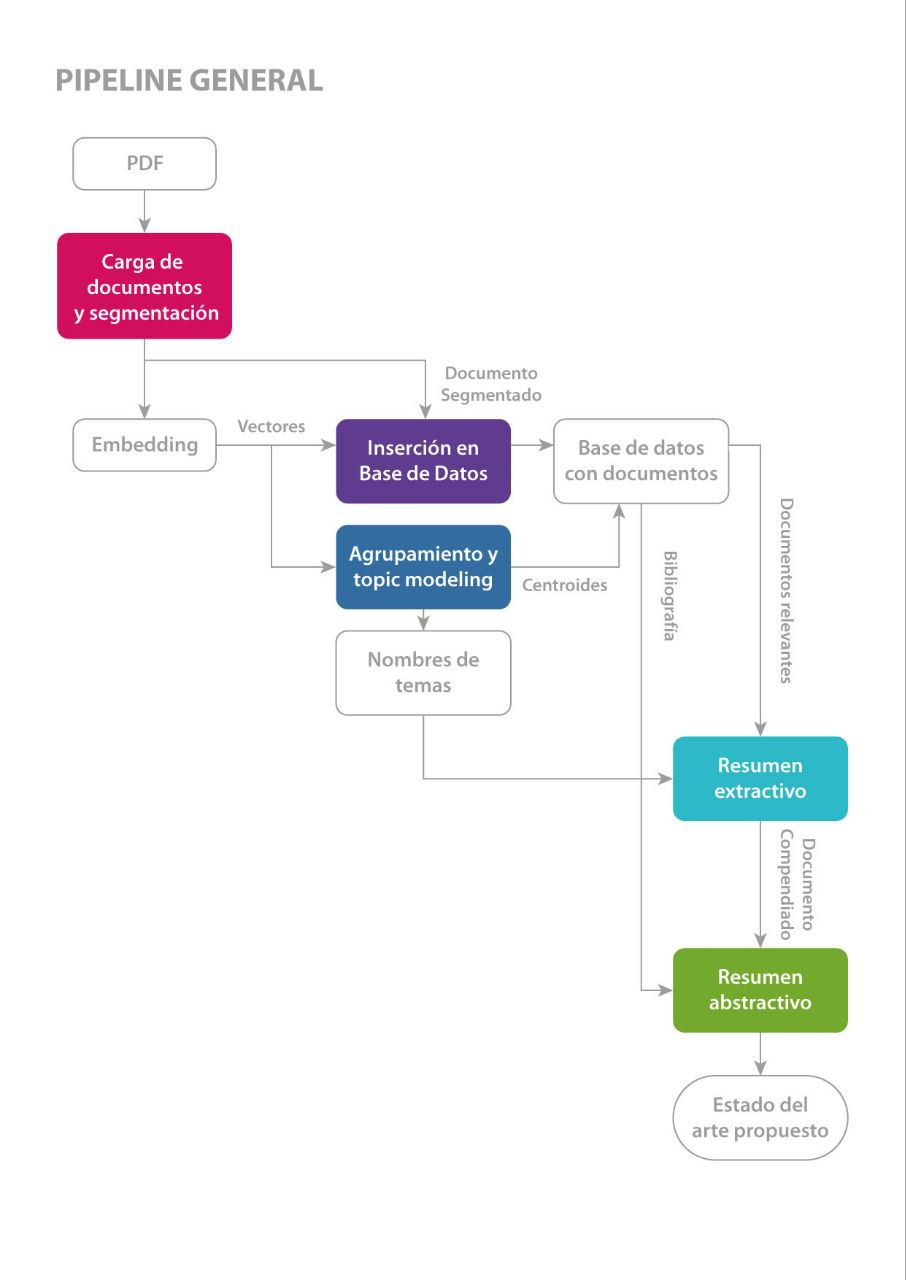
\includegraphics[scale = 1]{Figures/pipeline_general.png}
        \caption*{}
    \end{figure}
    

    \section{Primera fase: Carga de documentos} 
    La primera fase del \emph{pipeline} se centra en la carga los documentos. Se realiza además una segmentación de la información (en oraciones, párrafos u otro método de segmentación del texto) con el objetivo de representarla de manera granular. Con el fin de que sea más fácil agrupar semánticamente la información representada en los documentos. Esto será primordial para una fase posterior que se enfoca en la recuperación de la información.

    \begin{figure}[H]    
        \centering
        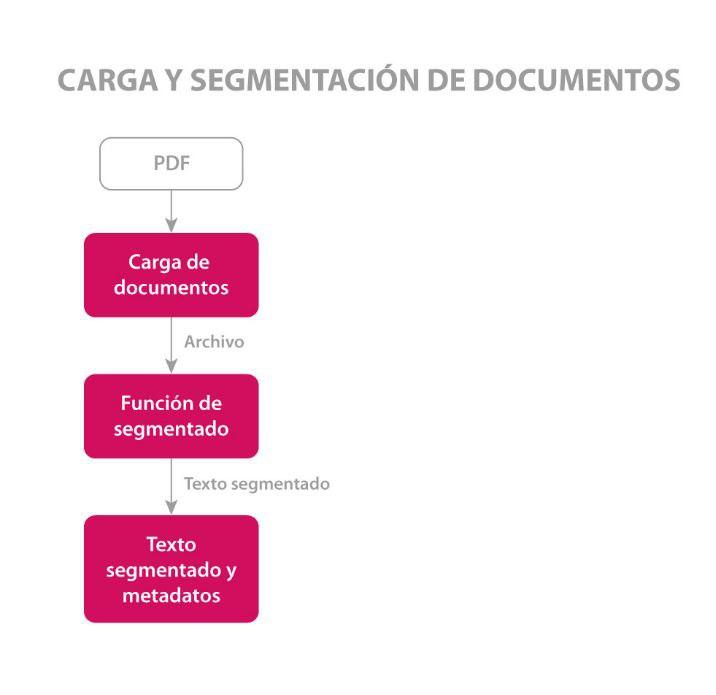
\includegraphics[scale = 1]{Figures/pipeline_1.png}
        \caption*{}
    \end{figure}
    
    \section{Segunda Fase: \emph{Embeddings}}
    Esta segunda fase comprende la conversión de la información previamente preprocesada en \emph{Embeddings de texto}.
    La representación del texto de esta manera permite obtener una abstracción de las ideas contenidas en los documentos. 
    Para ello se decidie utilizar el modelo `all-MiniML-L6-v2' que, de acuerdo con las pruebas de \emph{MTEB} [\cite{leaderboard}] obtiene buenos resultados sin altos requerimientos de tiempo y recursos computacionales. Estos \emph{embeddings} son unos vectores de dimensión 384 que serán almacenados en una base de datos vectorial para facilitar el acceso a estos y la realización de búsquedas por similaridad. \emph{Embedings} que traten del mismo tema se han de encontrar mas cerca entre si que \emph{embeddings} que representen conceptos diferentes.

    \begin{figure}[H]    
        \centering
        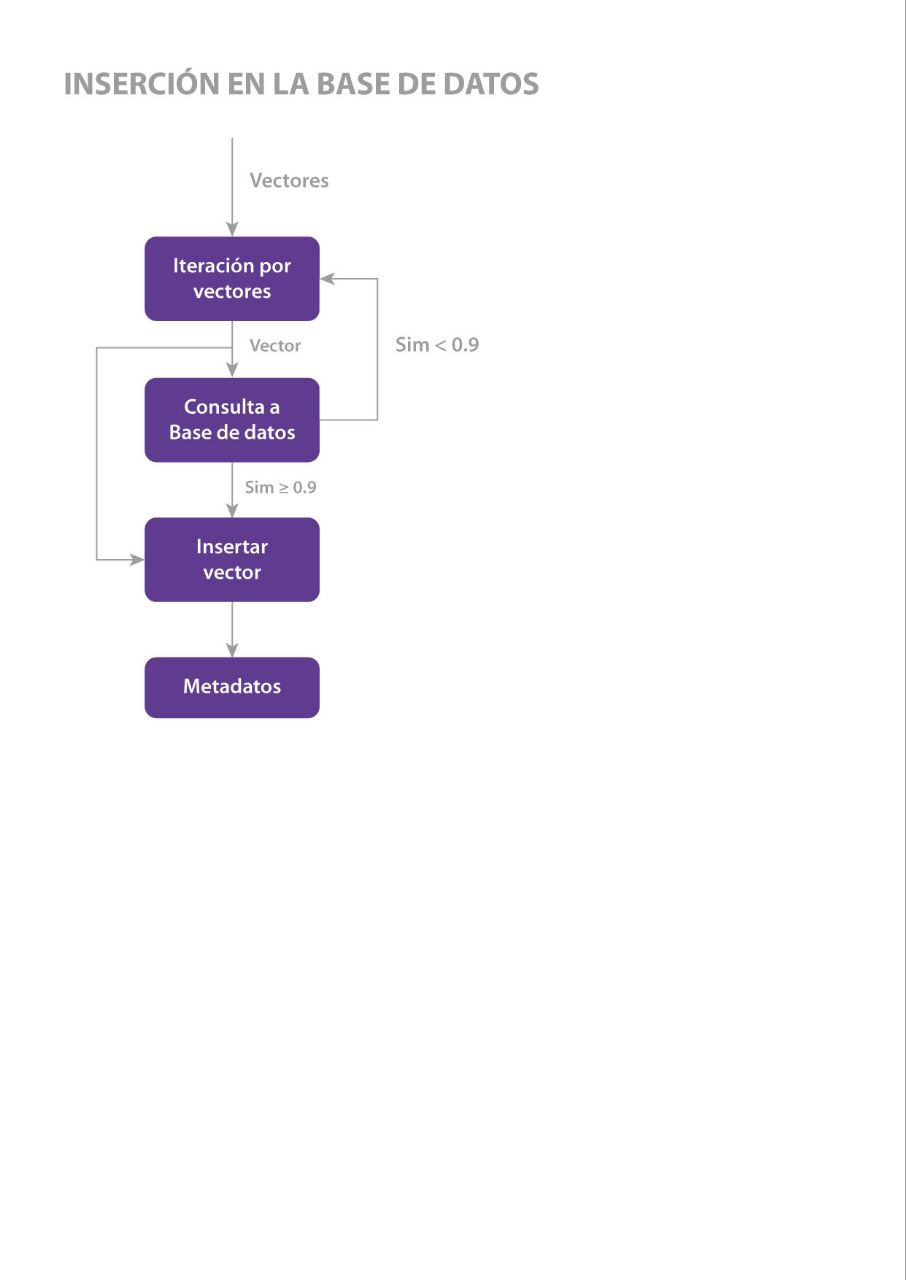
\includegraphics[scale = 1]{Figures/pipeline_2.png}
        \caption*{}
    \end{figure}

    \section{Tercera Fase: Inserción en la Base de datos}
    Los vectores que representan los documentos se almacenan en una base de datos vectorial que permite de manera eficiente acceder tanto a los documentos como a los metadatos de los mismos. A la vez que facilita el uso de búsqueda de similaridad utilizando otros vectores. Durante la inserción de los vectores se hace uso de esta funcionaliada para evitar introducir información redundante en la base de datos. De esta manera son descartados los vectores que no aportan información nueva a la base de conocimiento.

    \begin{figure}[H]    
        \centering
        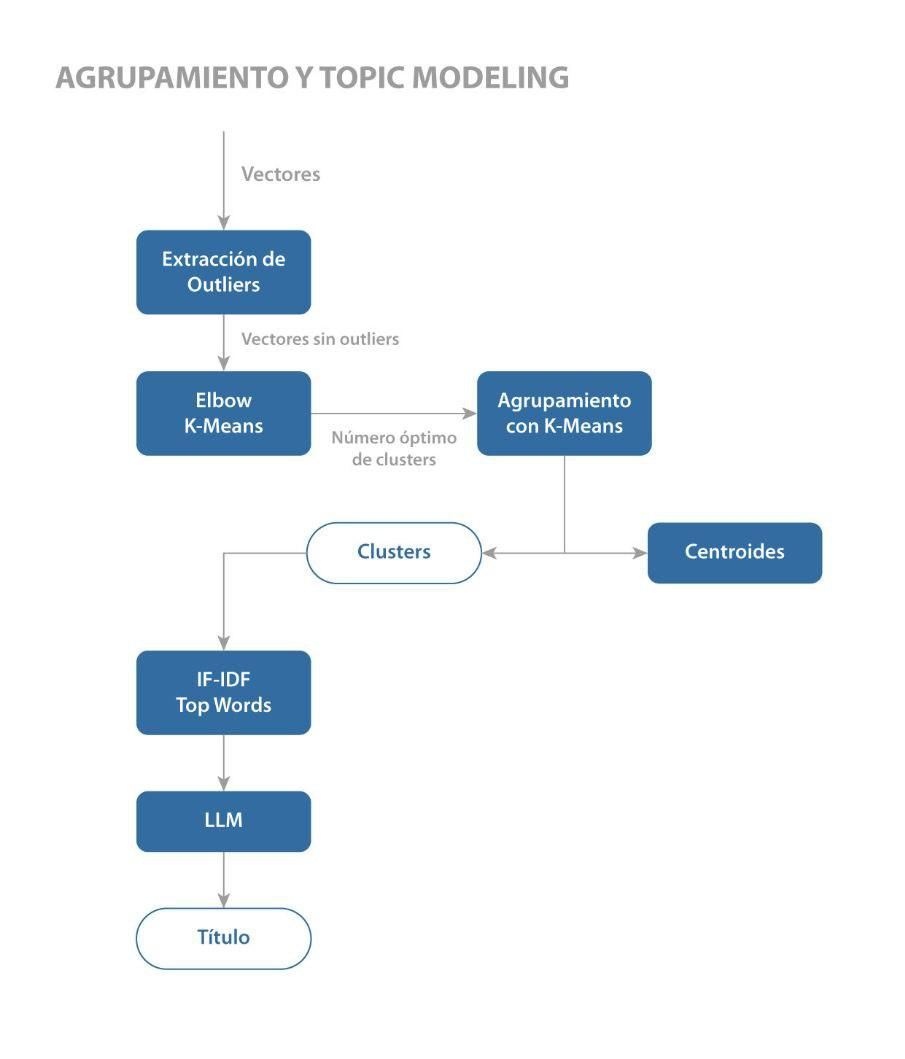
\includegraphics[scale = 1]{Figures/pipeline_3.png}
        \caption*{}
    \end{figure}

    \section{Cuarta Fase: Agrupamiento por temas}
    Una vez obtenidos los \emph{embeddings} es necesario agrupar la información en una serie de temas, para ello se procesan mediante un algoritmo de \emph{clustering} que se encarga de agruparlos atendiendo a la similaridad. Se hace uso del método del codo, una técnica utilizada en la clasificación de datos para determinar el número óptimo de clústeres\footnote{Un centroide es el punto representativo de un grupo de datos, calculado como el promedio de las características de todos los puntos pertenecientes a ese grupo, y se utiliza como el centro o punto focal para asignar datos a un clúster específico en algoritmos de agrupamiento.}. Este método se basa en calcular la distorsión promedio de cada clúster, que es la distancia de cada elemento con su centroide correspondiente. Al graficar la distorsión en función del número de clústeres, se busca identificar el punto donde la curva forma un "codo", indicando que agregar más clústeres no aportaría una mejora significativa. Una vez se obtiene la cantidad óptima de clústeres, se procede a generar un agrupamiento con todos los documentos y, por ende, los centroides que representan cada tema. Estos centroides están representados a su vez como vectores de la misma dimensionalidad que los \emph{embeddings} generados, por tanto; pueden ser utilizados para realizar una búsqueda en la base de datos vectorial que contiene los documentos. De esta manera se pueden recuperar los documentos que, conceptualmente estén más relacionados con el tema que los engloba. En esta fase además, una ves que se obtienen los distintos clústeres, se puedeutilizar una tabla \emph{TF-IDF} para obtener las palabras más relevantes para un tema. Con estas palabras, haciendo uso de un LLM se genera una propuesta de título para el tema.

    \begin{figure}[H]    
        \centering
        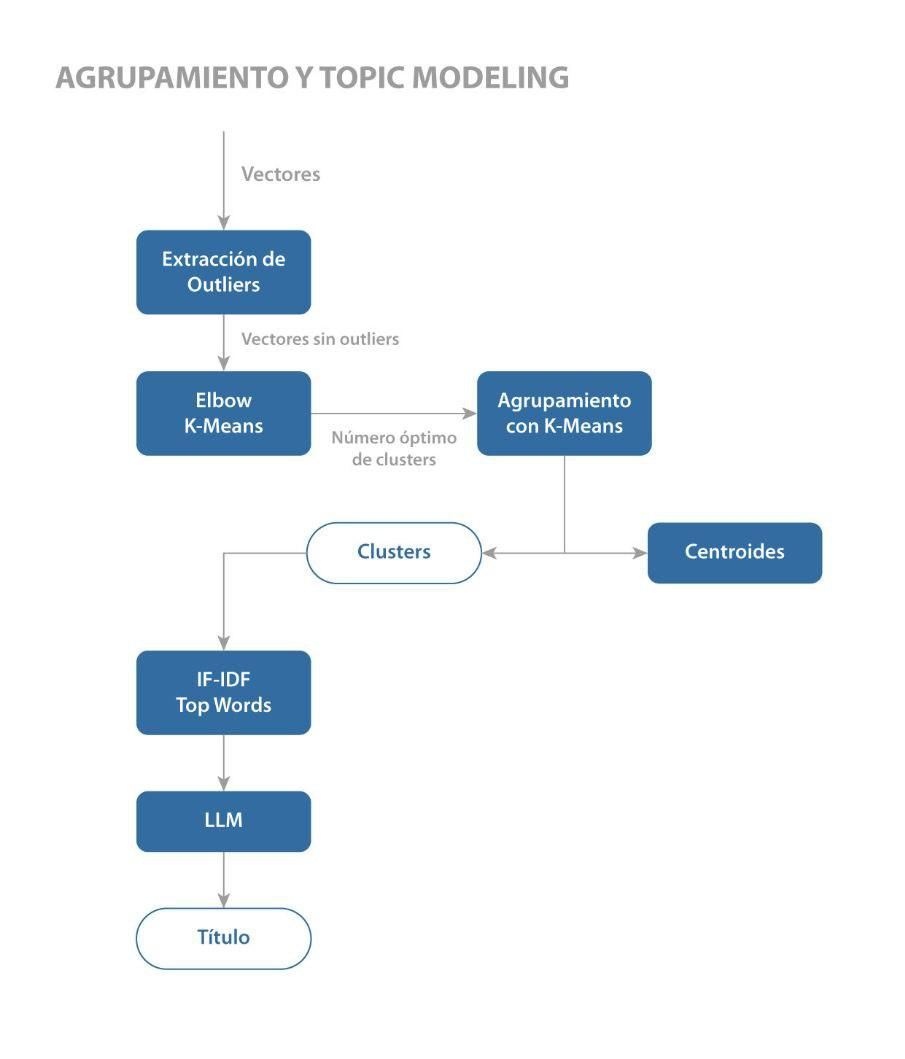
\includegraphics[scale = 1]{Figures/pipeline_3.png}
        \caption*{}
    \end{figure}

    \section{Quinta Fase: Resumen extractivo} 
    Los documentos más relevantes para un tema son recuperados tras realizar una búsqueda en la base de datos utilizando como referencia los centroides asociados a cada clúster. Estos documentos son agrupados a modo de resumen extractivo de cada uno de los temas detectados en el paso anterior (nótese que en este cointexto, un documento no necesariamente tiene que ser la totalidad del documento original, pues fueron segmentados en la primera fase). El proceso de extracción devuelve también los metadatos del elemento recuperado. Dichos metadatos actúan a modo de referencia al documento original que contiene la información de cada elemento recuperado por el sistema de bases de datos. De esta manera se garantiza una bibliografía consistente con la información recuperada. Estas referencias no serán procesadas por las futuras fases del \emph{pipeline}.
    
    \begin{figure}[H]    
        \centering
        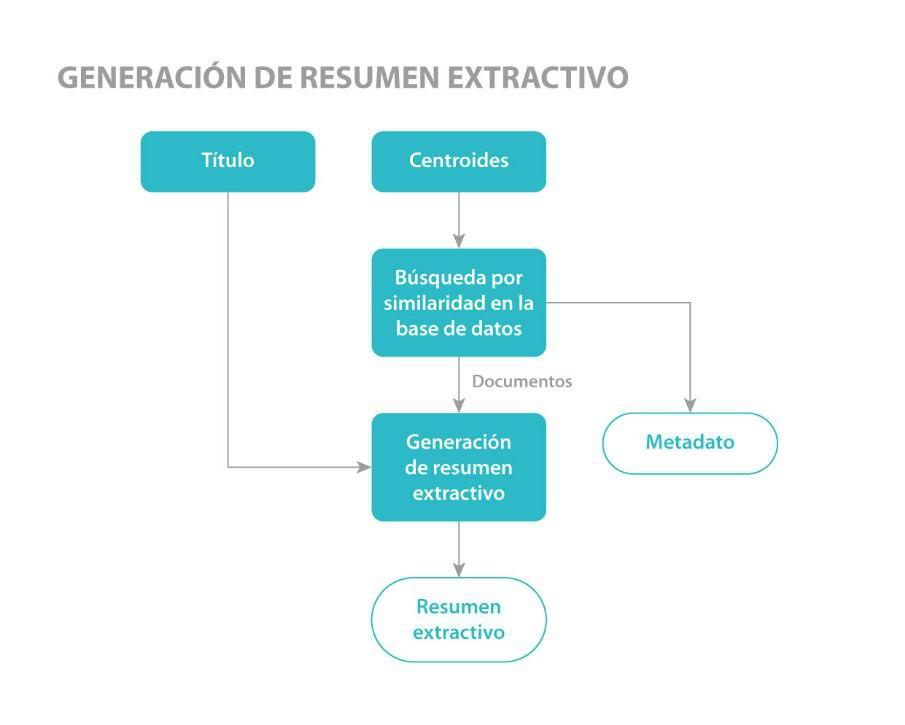
\includegraphics[scale = 1]{Figures/pipeline_4.png}
        \caption*{}
    \end{figure}

    \section{Sexta Fase: Resumen extractivo}
    El resumen extractivo generado en la fase anterior se utiliza como parte del \emph{prompt} que es utilizado por el LLM para generar el texto del resumen absrtactivo asociado a un tema.

    Los textos obtenidos son organizados acorde a un formato de salida predefinido: una enumeración de los temas definidos (con el título sugerido para el tema en la fase de agrupamiento por temas) y posteriormente el resumen correspondiente a cada tema. Se añaden también las referencias a los documentos utilizados obtenidos de la base de datos.

    \begin{figure}[H]    
        \centering
        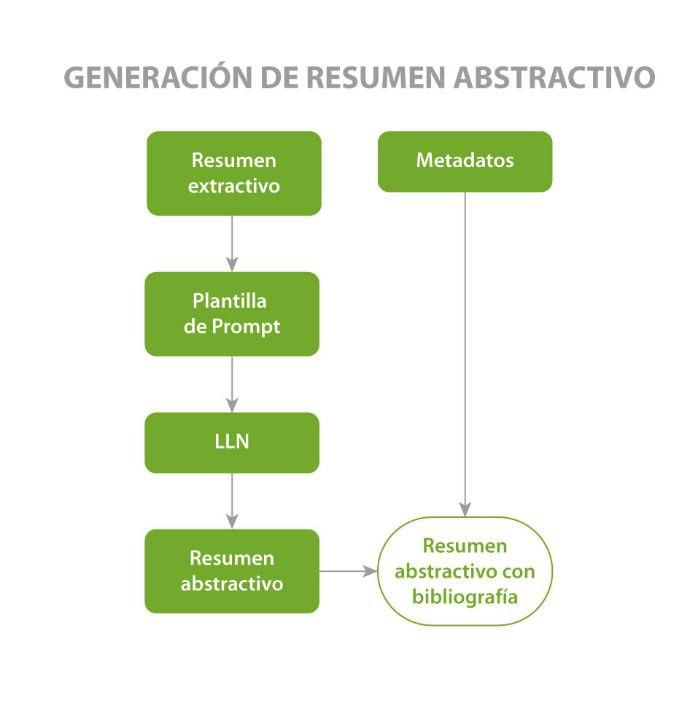
\includegraphics[scale = 1]{Figures/pipeline_5.png}
        \caption*{}
    \end{figure}

\chapter{Detalles de Implementación y Experimentos}\label{chapter:implementation}
En este capítulo se aborda la implementación de cada uno de los componentes que conforman el \´pipeline\´
descrito en este documento.

\section{Carga de documentos}
La carga de documentos se realiza haciendo uso de la biblioteca \code{langchain}[\cite{langchain}]
en particular el submódulo\code{PyPDFLoader} del módulo \code{document_loaders}, no obstante, este puede ser sustituido por otro módulo siempre que la respuesta cuente con campos \emph{metadata} y \emph{page_content}. En caso de sustituir completamente el módulo de carga de documentos se debe garantizar que el resultado de este primer paso sean dos listas, una con el texto de los documentos y otra con los metadatos de los mismos.
    \subsection{Segmentación del texto}
        Una de las limitaciones de los modelos de embedding y los \emph{LLMs} es la cantidad máxima de tokens\footnote{Un “token” se refiere a una unidad individual de significado en un texto.} que puede procesar de una vez, es por esto que es necesario, en los casos de documentos muy extensos, realizar una segmentación del texto para hacer un procesamiento parcial e independiente de las partes.
        En la implementación de este documento se ofreecen tanto la segmentación por oraciones como la segmentación por párrafos, no obstante algunos párrafos pueden ser demasiado extensos y saturar la capacidad máxima del modelo.

Una vez cargados los documentos y segmentados, se asocia cada segmento de texto con los metadatos correspondientes.

\section{Transformación a vectores}
    \subsection{Modelo para la generación de embeddings}
        En correspondencia con lo visto en el estudio del estado del arte, para la implementación de este pipeline se utilizó un grupo de modelos de generación de embeddings comprendidos entre las 15 primeras posiciones proporcionadas por \emph{MTEB}\cite{leaderboard} al momento de la revisión.

        Las dimensiones de los vectores generados por estos modelos de embedding varían entre los 1024, 768 y 384 elementos, además, la longitud de la secuencia que pueden procesar en todos los casos es de 512. Con este grupo de modelos de características diferentes se espera determinar si el desempeño de los modelos en esta tarea está directamente ligado a los resultados del modelo en \emph{MTEB} y evaluar cuán bien se desempeña un modelo más limitado en comparación con un modelo más extenso.

    Para la implementación del modelo de vectorización se creó una clase Embeddings que va a actuar a modo de \"wrapper\"\footnote{Un “wrapper” es un programa o código que encapsula y facilita el uso de otros componentes del programa} en la implementación proporcionada se utiliza la biblioteca langchain, particularmente el módulo de embeddings de HuggingFace para cargar los modelos de embeddings, se definen los métodos siguientes:
    \begin{enumerate}
        \item \emph{encode_many}: Método que recibe una lista de documentos y retorna una lista con los vectores resultantes de procesar dicho documento
        \item \emph{encode}: Método que recibe una cadena de texto y retorna el vector resultante de procesar el documento 
        \item \emph{get_model}: Método que retorna el modelo de embeddings que fue cargado. Esto es necesario para que tenga consistencia la búsqueda de similaridad de la base de datos
    \end{enumerate}

    Esta clase forma parte del pipeline, no obstante puede ser reemplazada por otra implementación que sea consecuente con el diseño descrito anteriormente.

    \subsection{Base de Datos Vectorial}
        \subsubsection{Selección del sistema de bases de datos}
            El sistema de bases de datos seleccionado para este proyecto es \emph{ChromaDB}\cite{chromadb}. Chroma DB es una base de datos vectorial que se destaca por su eficiencia en el almacenamiento y recuperación de incrustaciones de vectores. Permite la creación de colecciones, el filtrado de texto y la consulta de documentos similares, además de tener una excelente integración con python.
        Las interacciones con la base de datos se hacen a través de una clase que actúa a modo de \"wrapper\", esta vez con la siguiente estructura:
        \begin{enumerate}
            \item \emph{create_collection}: crea una nueva colección en la base de datos 
            \item \emph{get_collection}: retorna una colección, las operaciones re realizan sobre las colecciones
            \item \emph{list_collections}: retorna una lista con todas las colecciones existentes
            \item \emph{add} añade a la base de datos un nuevo documento, lo vectoriza utilizando el modelo de embeddings definido, si no se define ninguno, utiliza por defecto el modelo "all-MiniLM-L6-v2" de \emph{SentenceTransformers}, recibe como entrada el texto del documento y los metadatos.
            \item \emph{add_embedding_to_database}: añade un nuevo documento que ya haya pasado por el proceso de embedding,recibe como entrada el texto del documento, el vector que lo representa y los metadatos.
            \item \emph{add_embeddings}: añade un grupo de documentos ya vectorizados a la base de datos, recibe como entrada el texto del documento, los vectores y los metadatos. 
            \item \emph{query}: realiza una búsqueda de documentos relevantes para una consulta, la entrada será el texto  de la consulta y retorna los documentos relevantes, con vectores, texto y metadatos, la consulta es vectorizada por el modelo de embeddings definido.
            \item \emph{query_embeddings}: tiene un comportamineto similar a \emph{query} pero recibe en vez del texto a vectorizar, el vector que los representa; retorna los documentos relevantes (texto, vectores, metadatos)
        \end{enumerate}

        Todos los métodos de recuperación de información tienen un parámetro opcional \emph{top_k} que define la cantidad de documentos a retornar.

        Los métodos de inserción comprenden un mecanísmo que revisa si existen ya en la base de datos otros documentos que puedan ser redundantes con el nuevo documento que se desea insertar. La similaridad máxima permitida entre dos vectores es 0.9, no obstante este valor es modificable para tener un mayor control sobre el criterio de similaridad, en correspondencia con el modelo de embeddings que se utilice.

        Este módulo, como todos los demás del pipeline, es reemplazable por otros personalizados siempre y cuando sean consecuentes con la API\footnote{Una API (Interfaz de Programación de Aplicaciones) es un conjunto de definiciones y protocolos que permite a diferentes aplicaciones comunicarse entre sí y compartir información y funcionalidades.} descrita.

\section{Detección de temas}
    El proceso de detección de los temas (Topic Modelling) se realiza a través de un proceso de clustering\footnote{El clustering o análisis de agrupamiento es una técnica de aprendizaje no supervisado que agrupa un conjunto de datos en diferentes grupos o clusters} en el espacio de vectores que comprende los vectores que representan los documentos.

    \subsection{Algoritmo de Clustering}
        Para este proceso se utiliza el algoritmo K-Means Clustering, en particular la implementación que ofrece SKLearn\cite{sklearn} que además del algoritmo en sí, ofrece un método de detección automática de la cantidad óptima de clusters a través del método del codo[\cite{elbow}].
    
    Se implementó un wrapper para este proceso, el cual comprende los siguientes métodos:
    \begin{enumerate}
        \item \emph{generate_embeddings}: Método para procesar los documentos en caso de que no se proporcionen las versiones vectorizadas de estos, retorna la lista de vectores correspondiente a los embeddings de los documentos.
        \item \emph{detect_outliers}: Detecta los vectores que pueden ser considerados outliers\footnote{En estadística, un outlier es un punto de datos que difiere significativamente de otras observaciones} para evitar que estos afecten la correcta posición de los centroides.
        \item \emph{detect_optimal_k}: Detecta la cantidad óptima de agrupar los datos acorde al método del codo, la cantidad de grupos, por defecto se encuentra en el rango entre 2 y 15, no obstante estos valores pueden ser modificados a través de los parámetros \emph{lim_sub} y \emph{lim_sup} de la función.
        \item \emph{topic_words}: Retorna las palabras más repetidas en cada uno de los clusters; retira de la lista de palabras las que estan definidas en las stopwords de \emph{nltk}\footnote{Módulo Natural Language Toolkit https://www.nltk.org}
        \item \emph{get_topics}: Método principal que recibe los documentos, los procesa y extrae los outliers. Al grupo de documentos sin outliers les detecta el número óptimo de clusters; una vez detectado este número, realiza el proceso de clustering, esta vez con todos los documentos; de los clusters obtenidos, extrae las palabras representativas y, utilizando un \emph{LLM}, genera una sugerencia de título a partir de estas palabras. Este método retorna el centroide, las palabras más frecuentes y el título sugerido para cada cluster detectado.
    \end{enumerate}

    Este proceso genera una agrupación de los vectores de forma tal que se detectan distintos temas con los cuales asociar la información contenida en los documentos. Los centroides detectados están representados por vectores de la misma dimensionalidad que los vectores generados en en proceso de embedding; si se hiciera una representación en 2D del proceso descrito se obtendría una figura similar a \includegraphics{clustering2d.png} donde los puntos de colores simbolizan los documentos pertenecientes a cada tema y los puntos negros los centroides de cada uno de los temas.

    De esta manera si el centroide representa el punto que define la pertenencia de los documentos a un cluster que a su vez representa un tema, al obtenerse los documentos más relevantes con relación al vector que representa el centroide se estarán obteniendo los documentos más relevantes para el tema representado por dicho cluster, todo esto en correspondencia con la calidad de la representación vectorial del modelo de embeddings utilizado.
\section{Generación de los resúmenes}
    Una vez obtenidos los clusters se utilizan los centroides para recuperar los documentos más relevantes para cada tema. En este paso es importante tener en cuenta el método de segmentación de texto que se utilizó en el paso de carga de documentos. Este determinaría la cantidad de documentos a recuperar para, consecuentemente, no obtener una cantidad de documentos superior o inferior a la deseada, pues esto podría afectar la calidad de los resúmenes generados.
    
    Estos documentos recuperados, conforman un resumen extractivo preliminar, este resumen es entonces utilizado como parte del prompt de un \emph{LLM} para generar una abstracción del mismo. Efectivamente se obtiene una lista de los resúmenes de cada una de las secciones con las que se generará el estado del arte asociado a esos documentos, en correspondencia con la plantilla definida.
    Los documentos recuperados que son utilizados para generar el resumen de cada tema contienen en sus metadatos la información suficiente para ideintificar a qué archivo del corpus pertenecen, se añaden las referencias a estos documentos de origen utilizando esta infromación construyendo así las referencias bibliográficas del Estado del arte generado.

  

\section{Plantilla de Estado del Arte}
Se define la plantilla de Estado del arte como una plantilla que enumera los diferentes temas 
\section{Experimentación y Evaluación}

\backmatter

\begin{conclusions}
    El presente trabajo de grado ha introducido un modelo capaz de generar borradores de estados del arte utilizando un conjunto preseleccionado de documentos. Este modelo demuestra eficacia al producir un sistema de citaciones coherente con la información contenida en los documentos de entrada. Los resultados experimentales indican que es posible obtener un estado del arte sobre un tema específico en menos de 24 horas, lo cual aborda de manera efectiva la problemática asociada al tiempo que requiere realizar una investigación en la actualidad.

    Los experimentos realizados para validar el modelo con conjuntos de datos reales han arrojado resultados prometedores, respaldando la viabilidad y eficacia de la propuesta. No obstante, es imperativo reconocer las consideraciones especiales y limitaciones inherentes a esta investigación.
    
    Una limitación identificada radica en que, al pasar el sistema de citación por el \emph{LLM}, la consistencia se ve afectada, es por ello que se decide conservar la estructura generada por el resumen extractivo, provocando citas más extensas pero también mas precisas.
    
    Adicionalmente, se destaca la posible limitación del hardware para la implementación óptima del modelo. La exigencia de hardware especializado puede constituir un obstáculo, especialmente en relación con el factor tiempo. Esto puede llegar a implicar la imposibilidad de utilizar el modelo propuesto si no se cuenta con \emph{hardware} especializado.
    
    Durante la fase experimental, se observó que la cantidad y diversidad de los documentos influyen en las métricas del modelo. La significación de esta variabilidad en los resultados requiere una evaluación más detallada.
    
    En conclusión, aunque este trabajo representa un avance sustancial en la automatización de la generación de estados del arte, se reconoce la necesidad de abordar las limitaciones mencionadas. Estas consideraciones ofrecen oportunidades para futuras investigaciones y mejoras.
\end{conclusions}

\begin{recomendations}
    Se plantea como sugerencias fundamentales para futuras investigaciones la creación de conjuntos de datos específicos que superen las limitaciones actuales de los datos públicos, centrándose especialmente en la expansión del texto y la diversificación de las fuentes. Se aboga por la inclusión de conocimientos no científicos e información multilingüe con el objetivo de enriquecer la calidad de los conjuntos de datos. También se propone realizar un estudio cuantitativo para evaluar cómo la diversidad de contenido y el número de documentos impactan la calidad de los resúmenes, investigando posibles desviaciones en las métricas de evaluación.

    Además, se recomienda encarecidamente el desarrollo de una implementación que fomente una mayor interacción del usuario, concediéndole la capacidad de solicitar modificaciones en el documento ya sea total o parcialmente según su criterio. Esta recomendación incluye la implementación de una interfaz gráfica intuitiva y la integración de funcionalidades de preguntas y respuestas referentes a los documentos, con el propósito de mejorar la experiencia y brindar mayor control sobre el contenido generado.
    
    Asimismo, se destaca la importancia de asegurar el soporte a varios formatos de salida establecidos, como Latex, JSON, entre otros. Esta medida busca adaptarse a las diversas necesidades de los usuarios y facilitar la interoperabilidad con otras herramientas y plataformas. Estas recomendaciones se presentan como contribuciones esenciales para avanzar en el desarrollo de herramientas de resumen de texto más efectivas y versátiles.
\end{recomendations}

\include{BackMatter/Bibliography}

\end{document} 